\section{This generic framework applied to \ac{bus} imaging.}

In this section, the generic framework presented in the previous section is applied to \ac{bus} imaging. We need to define our problem properly. 

\subsection{Problem formulation for segmentation of \ac{bus} imaging.}

We recall that the aim in segmentation is to affect to a discrete set of elements $\mathcal{S}$, a label $l$ from a labelling set $\mathcal{L}$. In our case, our labelling set $\mathcal{L} = \{ \text{chest wall}, \text{lungs}, \dots, \text{lesion} \}$ (see \Cref{fig:methodTerms:problem} for the entire set of labels) and the set $\mathcal{S}$ is chosen to be a super-pixels representation of the image~\cite{achanta2012slic}. In our case, $\mathcal{S}$ is the result from an over-segmentation of the image using Quick-shift super-pixel. \Cref{fig:methodTerms:problem} illustrates one such representation $\mathcal{S}$, applied to a \ac{bus} image example. The super-pixels are coloured according to the image's \ac{gt}. Bear in mind that given an unseen \ac{bus} image, the ultimate goal is to represent the image as a set of super-pixels and infer the appropriated labelling for each of them.

\subsection{Data term definition for segmentation of \ac{bus} imaging.} \label{sec:method:dterm:feat}

\begin{figure}
    \centering
    \begin{subfigure}[b]{0.30\textwidth}
        \centering
        \begin{tikzpicture}
          \node[inner sep=0, draw] (breast) {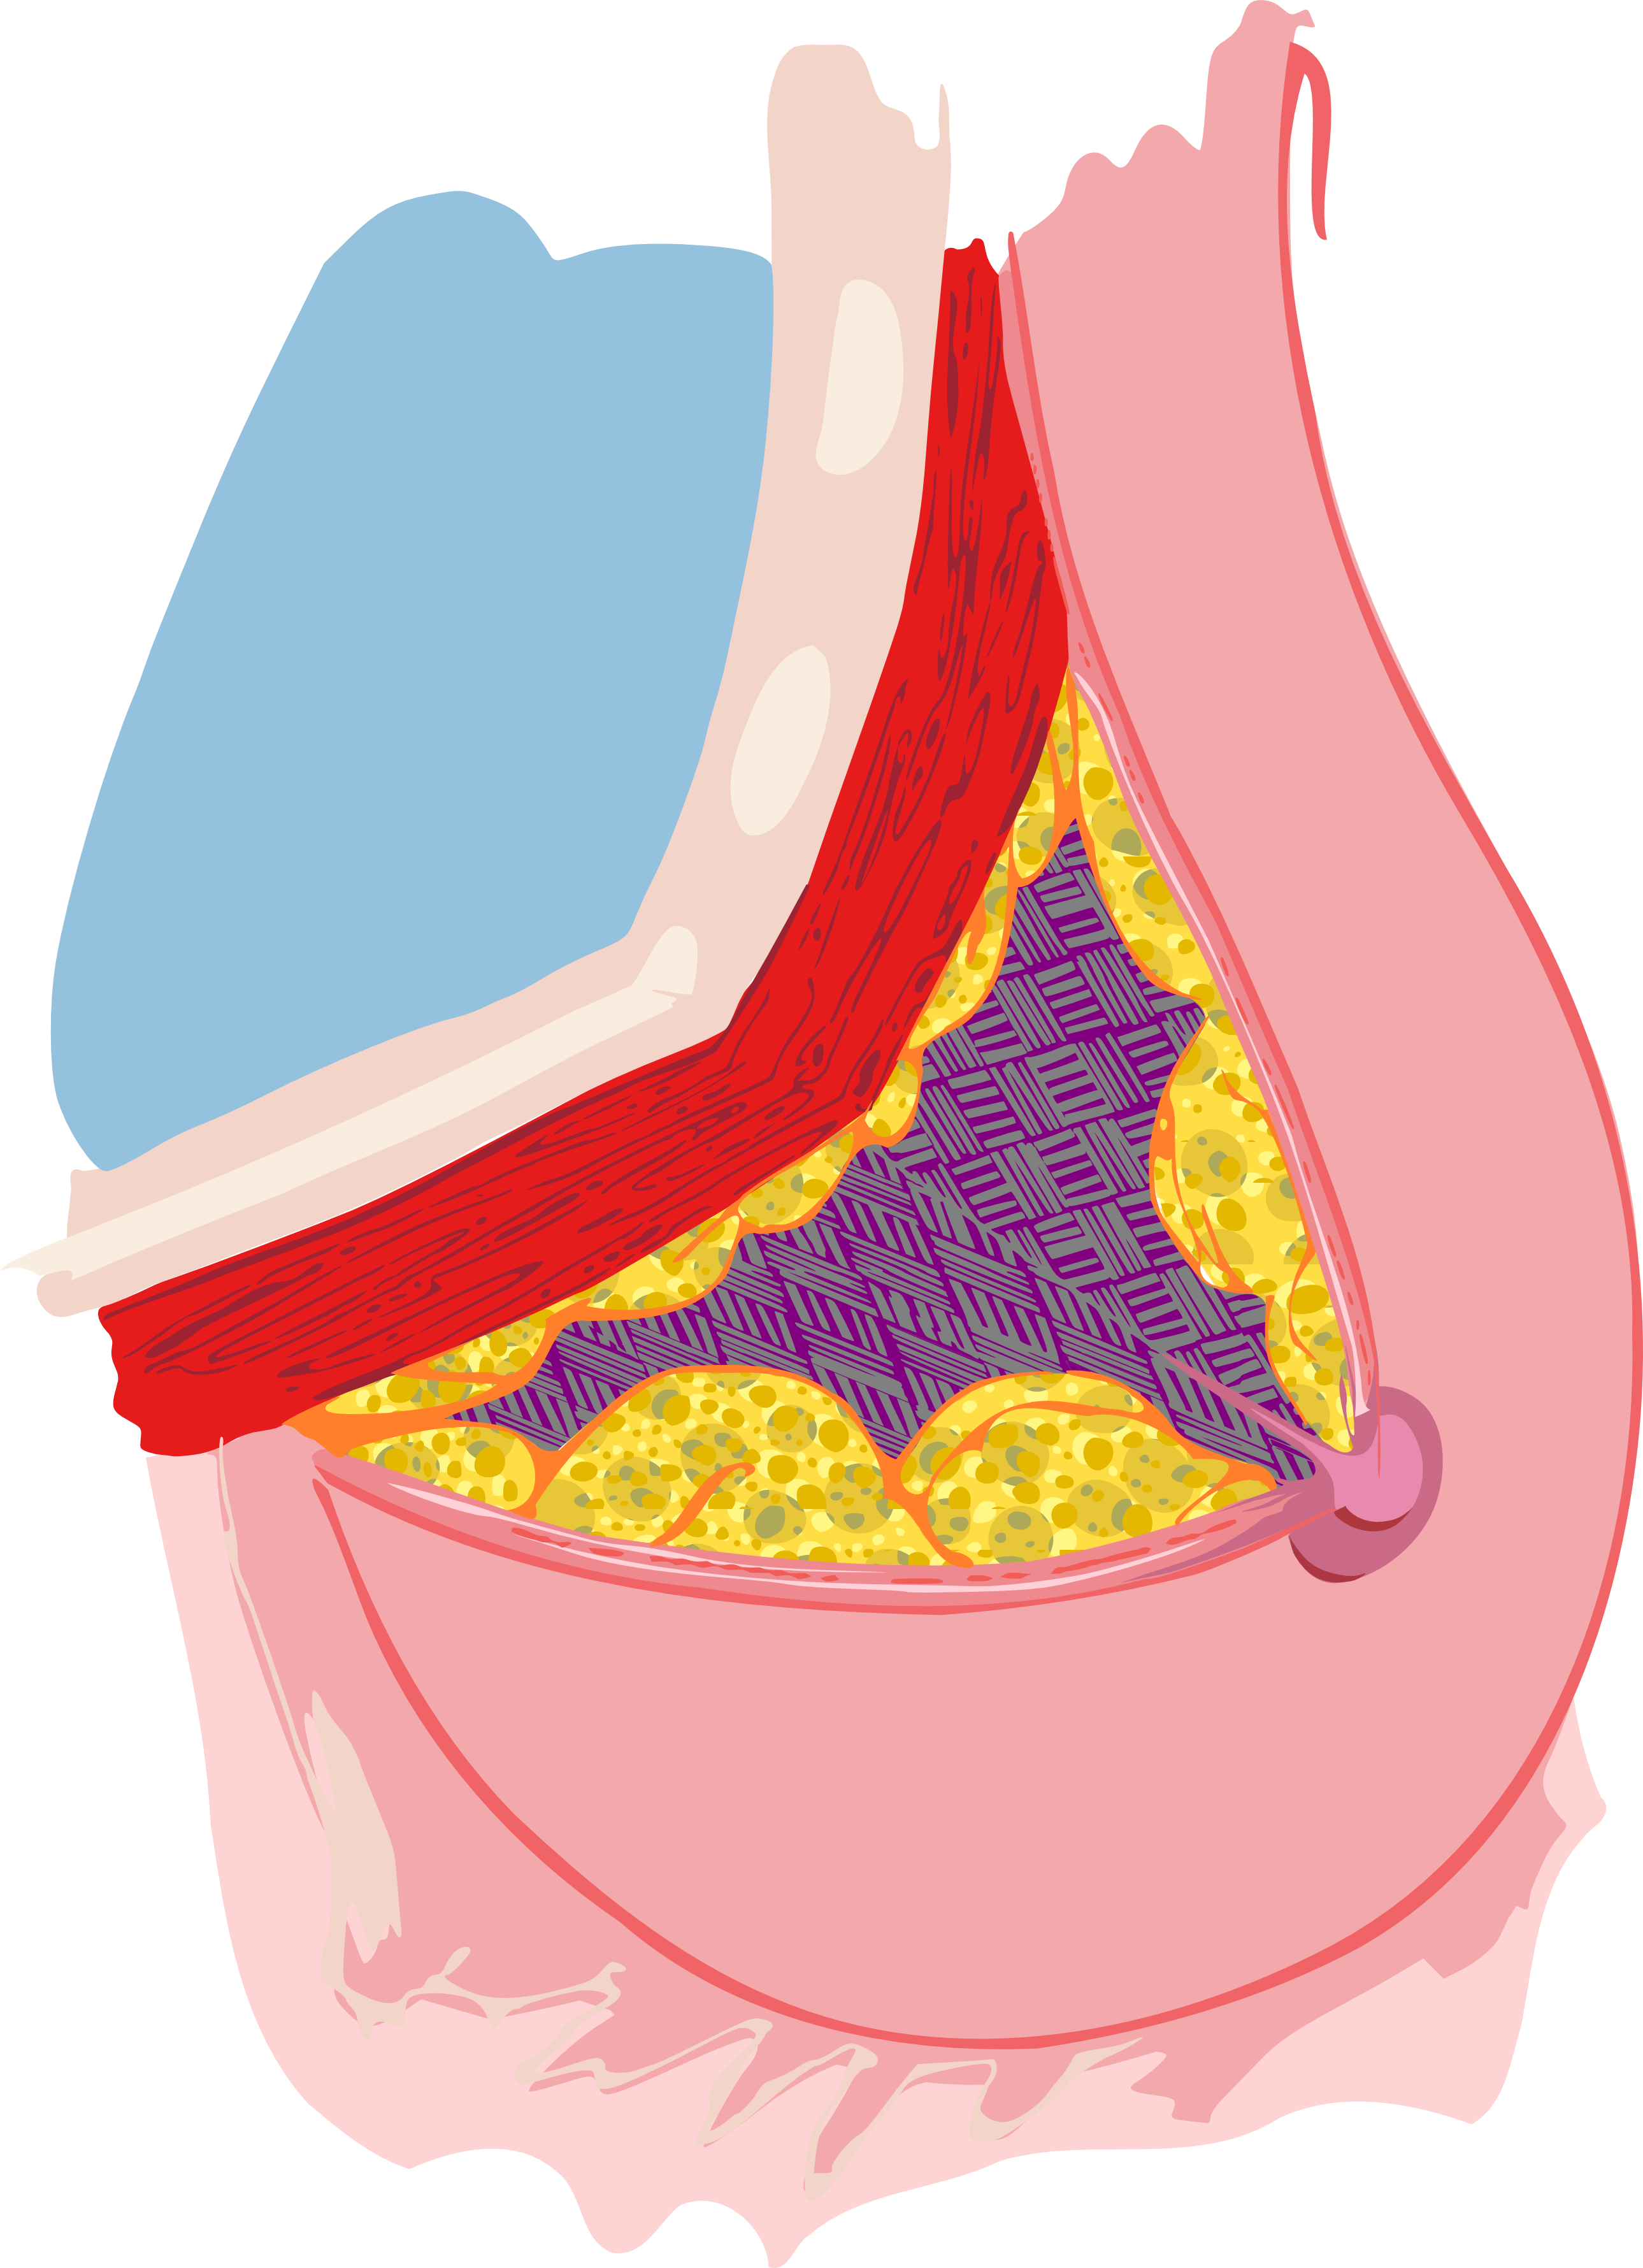
\includegraphics[width=0.4\textwidth]{breast}};
          \node[inner sep=0, draw, below= 2pt of breast] (slice) {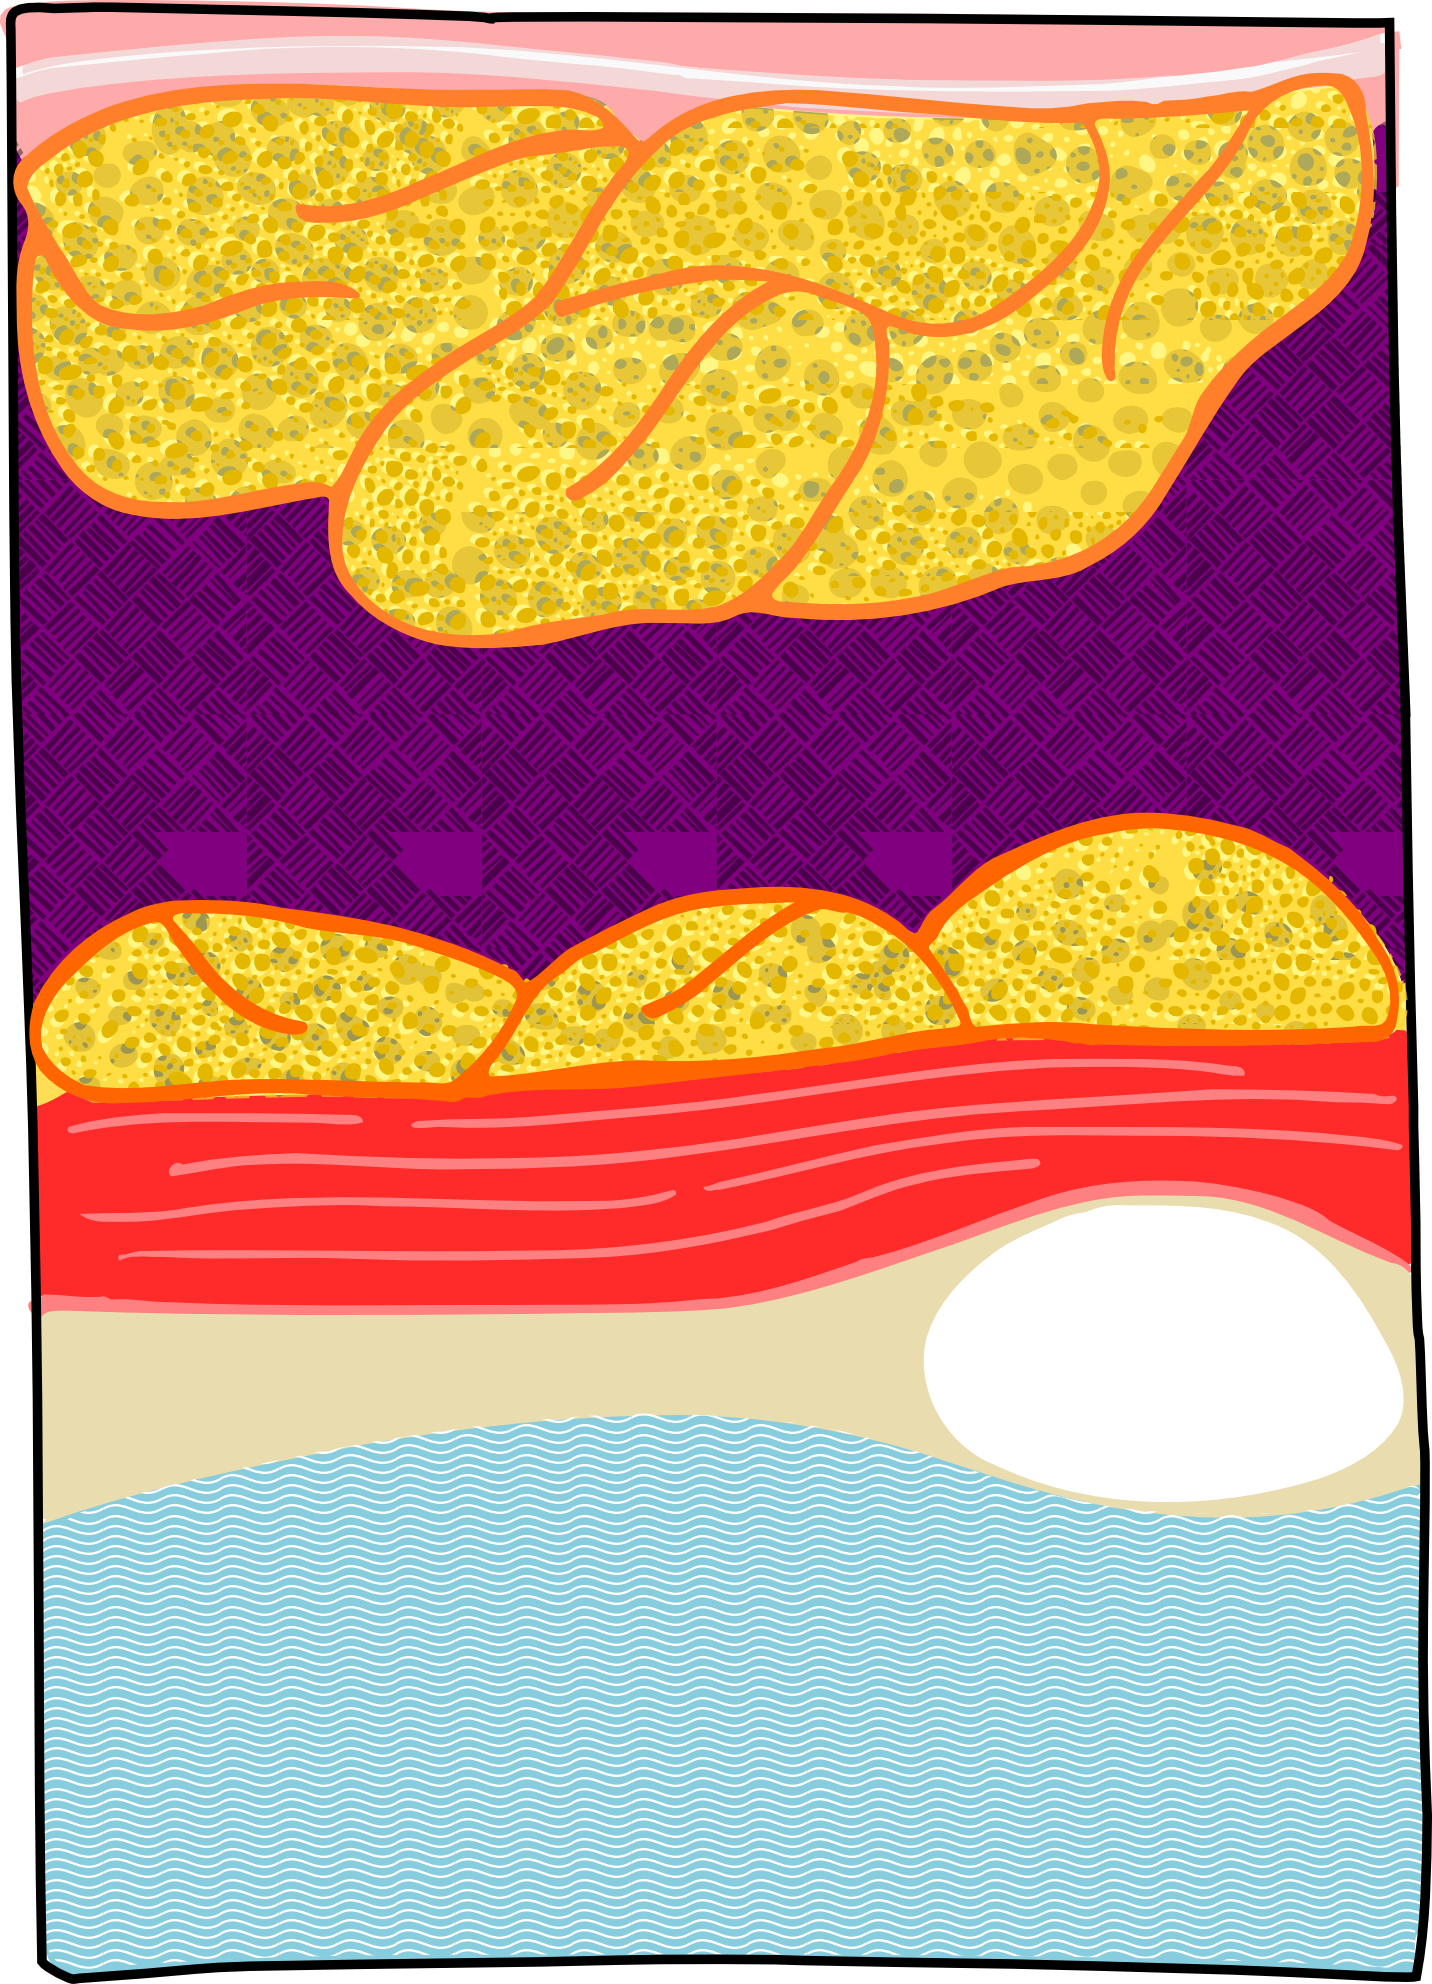
\includegraphics[width=0.4\textwidth]{slice}};
        \end{tikzpicture}
        %\caption{{\small Breast structure}}    
        \label{fig:features:breast}
    \end{subfigure}
    \hfill
    \begin{subfigure}[b]{0.34\textwidth}   
        \centering 
        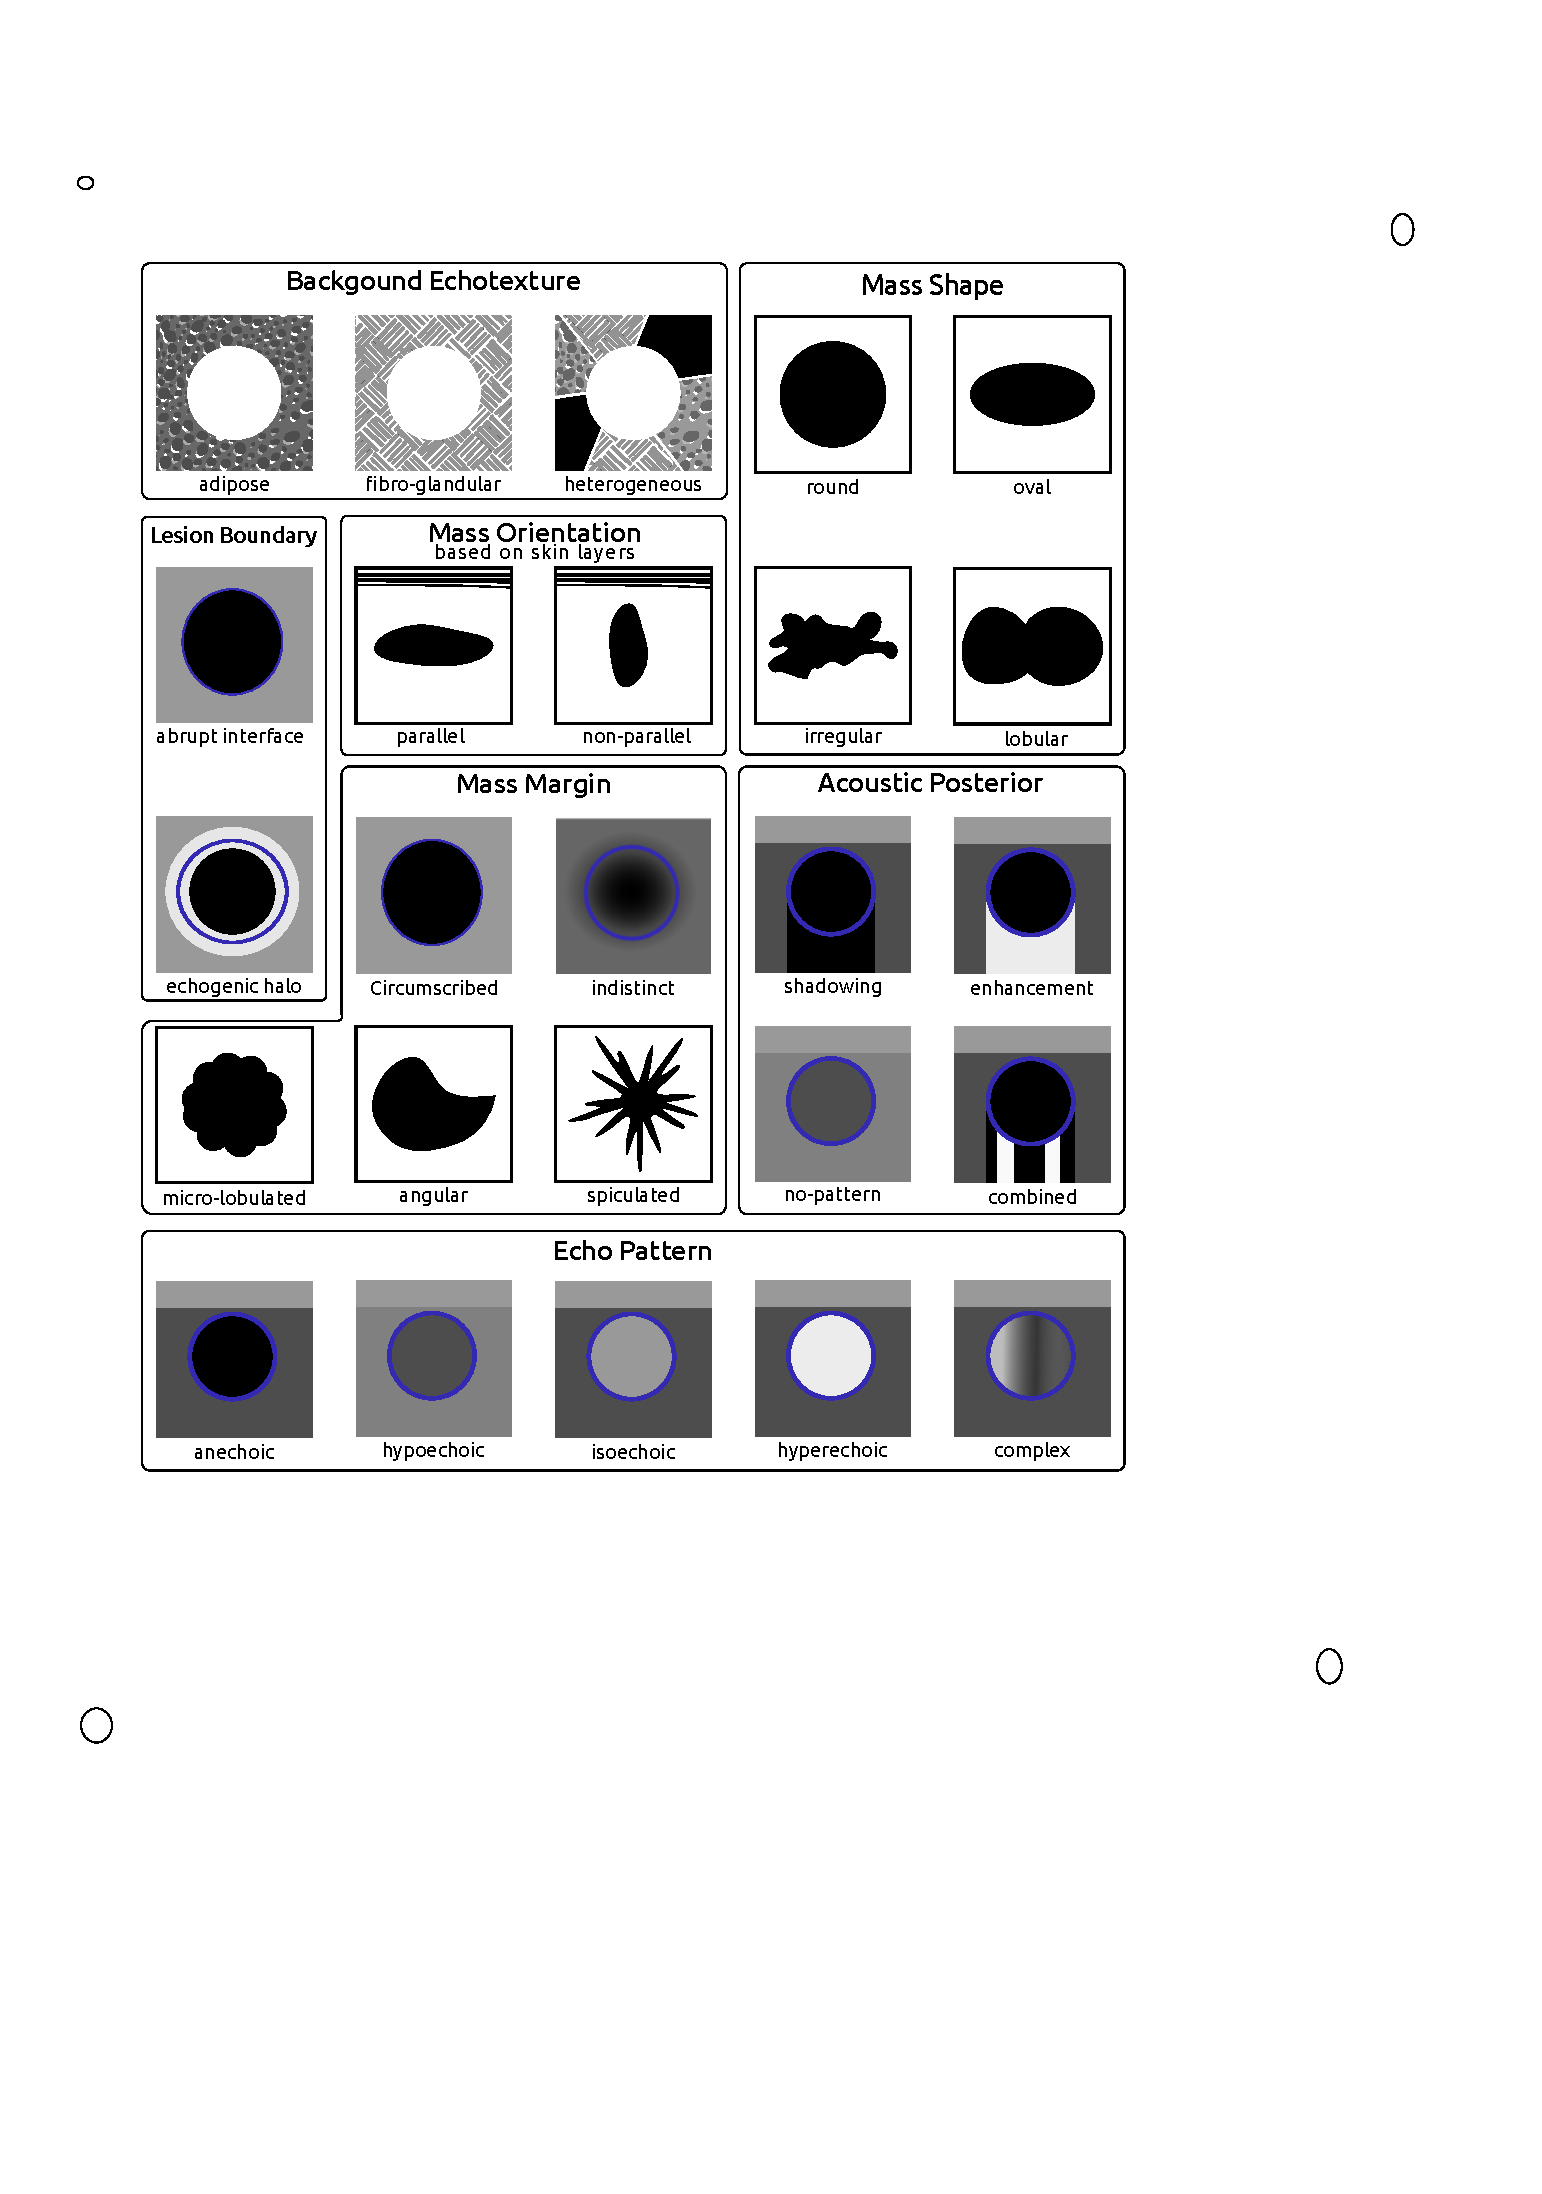
\includegraphics[trim = 65 345 200 124, clip,width=0.9\textwidth]{birads}
        %\caption[]%
        %{Breast lesion characteristics in \ac{us} screening influencing clinical management~\cite{biradsus}}    
        \label{fig:features:lexicon}
    \end{subfigure}
    \hfill
    \begin{subfigure}[b]{0.2\textwidth}
      \newcommand{\insertVisualCue}[2]{
        \tikz{\node[label=above:#2]{\includegraphics[width=0.3\textwidth]{#1}};}
      }
      \centering
      \begin{tiny}
        \insertVisualCue{AppearanceCues}{Appearance}
        \vfill
        \insertVisualCue{AtlasCues}{{Atlas, Brightness}}
        \vfill
        \insertVisualCue{siftCues}{SIFT-BoF}
      \end{tiny}
      %\caption{Visual cues encoded in the features}
      \label{fig:features:relation}
    \end{subfigure}
    \hfill
    \caption {{\footnotesize Visual reference: (a) breast structures, (b) US BI-RADS lexicon, (c) encoded visual cues.}} 
    \label{fig:features}
\end{figure}

\subsubsection{Features generation based on visual cues}

The structures of the breast and their rendering when using a hand-held 2D \ac{us} probe are sketched in \cref{fig:features:breast}. \Cref{fig:features:lexicon} illustrates the lexicon proposed by the \ac{acr}~\cite{biradsus} and used by clinicians to perform their diagnosis. Thus, our aim is to generate a set of computer vision features which is able to encode the characteristic described in the lexicon. Thus, \cref{fig:features:relation} depicts the relations between the visual clues of the lexicon and the computer vision features selected. These features can be summarized as:

\begin{description}
  \item[Appearance] 
    Based on the multi-labelled \ac{gt}, a \ac{mad} histogram model for every tissue label is built. The Appearance feature is computed as the $\chi^2$ distance between a histogram of $s$ and the models generated.
  \item[Atlas] 
    Based on the multi-labelled \ac{gt} an atlas is build to encode the labels likelihood based on the location of $s$.
  \item[Brightness] 
    Intensity descriptors are computed based on statistics of $s$ (\emph{i.e:} mean, median, mode) and  are compared with some intensity markers of the set $\mathcal{S}$ such as the minimum intensity value, the maximum, its mean, etc.
  \item[\ac{sift}-\ac{bof}]
    $s$ is described as an histogram of visual words based on \ac{sift}~\cite{massich2014sift}. The dictionary is built with $36$ words.
\end{description}

In order to incorporate multi-resolution, each super-pixel is group with its adjacent super-pixels such that $s' = \{s \cup \mathcal{N}_{s}\}$, the features are recalculated using $s'$ and concatenated to the original feature descriptor of $s$.
This operation can be repeated several times.

The B.Echo-texture, is mainly encoded by the SIFT-BoF but also through the Appearance feature since elements would have the same model.
Acoustic Posterior is mainly captured by the Brightness feature, but the Atlas also brings crucial information to compensate for intensity inhomogeneities caused by signal attenuation present in the most posterior parts of the image.
The Echo Pattern cue, encodes the echogenity of a region with respect to the adipose tissue. This can be found at the anterior part of the image with its echogenity close to the middle of the spectrum. Appearance, Brightness and the Atlas account for such information.

However, it can be notice that not all the visual cues compiled in the lexicon are suitable to be encoded by the features.
Mass shape, orientation and margin cues do not characterize an individual super-pixel but a group of contiguous super-pixels sharing the same label.
Characterising super-pixels in those terms imply that super-pixels should be image elements of the same order as the lesions. 
This is not the case, since the bottom-line is to aggregate small regions to form the segmentation.
The lesion boundary cue falls at the other extreme.
To encode this visual cue as features implies to use smaller super-pixels in order to be fully contained within the halo, limiting the discriminatory power of other features that need larger regions to build higher-level descriptors.

\subsubsection{Encoding the data term}

 A choice regarding the encoding of the data term has to be made by using a \ac{ml} classifier. An \ac{svm} classifier  with an \ac{rbf} kernel is selected to determine the data model during the training stage. During the testing stage, $D_s(\omega_s=l)$ corresponds to the distance between the testing samples and the model associated with $l$ as the \ac{svm} classification reward. 

\subsection{Pairwise term definition for segmentation of \ac{bus} imaging.}

The pairwise term is our framework was defined as in \cref{eq:smoothing}.

\subsection{Optimization of our cost function.}

The optimization used to solver our cost function $U(\cdot)$ is \ac{gc}. \ac{gc} when applicable allows to rapidly find a strong local minima guaranteeing that no other minimum with lower energies can be found~\cite{delong2012fast}. 
\ac{gc} is applicable if, and only if, the pairwise term favours coherent labelling configurations and penalizes labelling configurations where neighbours labels differs; 
such is our case, given by \cref{eq:smoothing}.

%%% Local Variables: 
%%% mode: latex
%%% TeX-master: "../../master"
%%% End: 
